%
% teil3.tex -- Resultate und Ausblick
%
% (c) 2022 Fabian Dünki, Hochschule Rapperswil
%
\section{Auswertung
\label{0f1:section:teil3}}
\rhead{Resultate}
Im Verlauf dieser Arbeit hat sich gezeigt, 
das einen einfachen mathematischen Algorithmus zu implementieren gar nicht so einfach ist.
So haben alle drei umgesetzten Ansätze Probleme mit grossen negativen $z$ in der Funktion $\mathstrut_0F_1(;c;z)$.
Ebenso kann festgestellt werden, dass je grösser der Wert $z$ in $\mathstrut_0F_1(;c;z)$ wird, desto mehr weichen die berechneten Resultate von den Erwarteten \cite{0f1:wolfram-0f1} ab.

\subsection{Konvergenz
\label{0f1:subsection:konvergenz}}
Es zeigt sich in Abbildung \ref{0f1:ausblick:plot:airy:konvergenz}, dass nach drei Iterationen ($k = 3$) die Funktionen genaue Resultate im Bereich von $-2$ bis $2$ liefert. Ebenso kann festgestellt werden, dass der Kettenbruch schneller konvergiert und im positiven Bereich sogar mit der Referenzfunktion $\operatorname{Ai}(x)$ übereinstimmt. Da die Rekursionsformel eine Abwandlung des Kettenbruches ist, verhalten sich die Funktionen in diesem Fall gleich.

Erst wenn mehrerer Iterationen gemacht werden, um die Genauigkeit zu verbessern, ist der Kettenbruch den anderen zwei Algorithmen bezüglich Konvergenz überlegen. 
Interessant ist auch, dass die Rekursionsformel nahezu gleich schnell wie die Potenzreihe konvergiert, aber sich danach, wie in Abbildung \ref{0f1:ausblick:plot:konvergenz:positiv} zu beobachten ist, einschwingt. Dieses Verhalten ist auch bei grösseren $z$ zu beobachten, allerdings ist dann die Differenz zwischen dem ersten lokalen Minimum von $k$ bis zum Abbruch kleiner.
Dieses Phänomen ist auf die Lösung der Rekursionsformel \eqref{0f1:math:matrix:ende:eq} zurück zu führen. Da im Gegensatz die ganz kleinen Werte nicht zu einer Konvergenz wie beim Kettenbruch führen, sondern sich noch eine Zeit lang durch die Multiplikation aufschwingen.

Ist $z$ negativ wie in Abbildung \ref{0f1:ausblick:plot:konvergenz:negativ}, führt dies zu aufgrund des Vorzeichens zu alternierenden Termen. So steigt bei allen Algorithmen zuerst die Differenz zum erwarteten Endwert. Erst nach genügend Iterationen sind die Terme genügend klein, so dass sie das Endresultat nicht mehr signifikant beeinflussen.
Auch hier konvergiert der Kettenbruch am schnellsten von allen Algorithmen. Ebenso bricht die Rekursionsformel nahezu gleichzeitig mit der Potenzreihe ab.

\subsection{Stabilität
\label{0f1:subsection:Stabilitaet}}
Verändert sich der Wert von $z$ in $\mathstrut_0F_1(;c;z)$ gegen grössere positive Werte, wie zum Beispiel $c = 800$ liefert die Kettenbruch-Funktion (Listing \ref{0f1:listing:kettenbruchIterativ}) \verb+inf+ zurück. Dies könnte durch ein Abbruchkriterien abgefangen werden. Allerdings würde das, bei grossen Werten zulasten der Genauigkeit gehen. Trotzdem könnte, je nach Anwendung, auf ein paar Nachkommastellen verzichtet werden.

Wohingegen die Potenzreihe (Listing \ref{0f1:listing:potenzreihe}) das Problem hat, dass je mehr Terme berechnet werden, desto schneller wächst die Fakultät im Nenner. Dies führt zu einer Bereichsüberschreitung des \verb+double+ Bereiches \cite{0f1:double}, der spätesten ab $k=167$ eintritt. Schlussendlich gibt das Unterprogramm das Resultat \verb+-nan(ind)+ zurück.
Die Rekursionformel \eqref{0f1:listing:kettenbruchRekursion} liefert für sehr grosse positive Werte die genausten Ergebnisse, verglichen mit der GNU Scientific Library. Wie schon vermutet ist die Rekursionsformel, im positivem Bereich, der stabilste Algorithmus. Um die Konvergenz zu gewährleisten, muss wie in Abbildung \ref{0f1:ausblick:plot:konvergenz:positiv} dargestellt, die Iterationstiefe $k$ genug gross gewählt werden.

Im negativem Bereich sind alle gewählten und umgesetzten Ansätze instabil. Grund dafür ist die Potenz von $z$, was zum Phänomen der Auslöschung \cite{0f1:SeminarNumerik} führt. Schön zu beobachten ist dies in der Abbildung \ref{0f1:ausblick:plot:airy:stabilitaet} mit der Airy-Funktion als Test. So sind sowohl die Potenzreihe, der Kettenbruch, als auch die Rekursionsformel bis ungefähr $\frac{-15^3}{9}$ stabil. Dies macht auch Sinn, da alle Algorithmen auf der gleichen mathematischen Grundlage basieren. Danach verhält sich allerdings die Instabilität unterschiedlich. Diese programmiertechnischen Unterschiede sind auch in Abbildung \ref{0f1:ausblick:plot:konvergenz:positiv} und \ref{0f1:ausblick:plot:konvergenz:negativ} festzustellen.

\begin{figure}
    \centering
    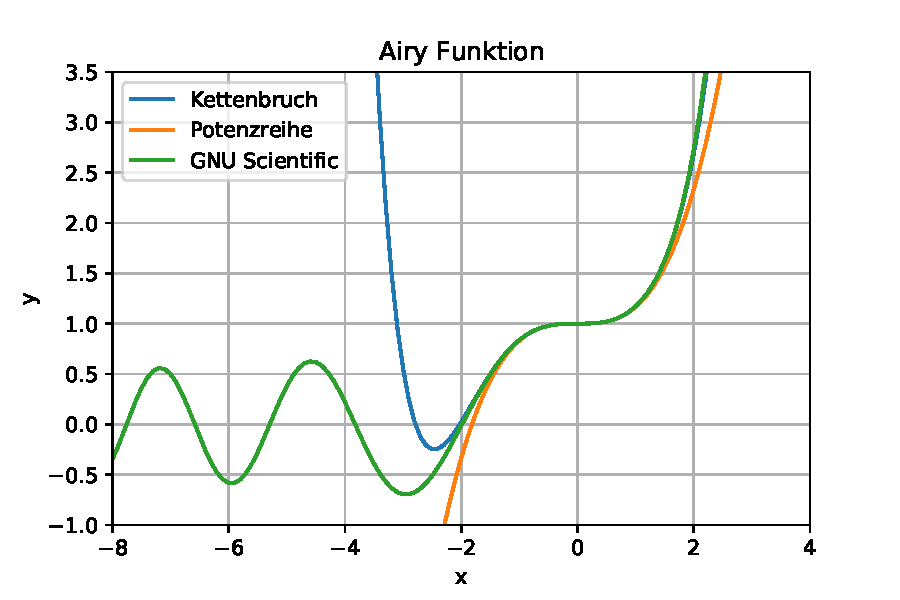
\includegraphics[width=0.8\textwidth]{papers/0f1/images/konvergenzAiry.pdf}
    \caption{Konvergenz nach drei Iterationen, dargestellt anhand der Airy Funktion zu den Anfangsbedingungen $\operatorname{Ai}(0)=1$ und $\operatorname{Ai}'(0)=0$.
    \label{0f1:ausblick:plot:airy:konvergenz}}
\end{figure}

\begin{figure}
    \centering
    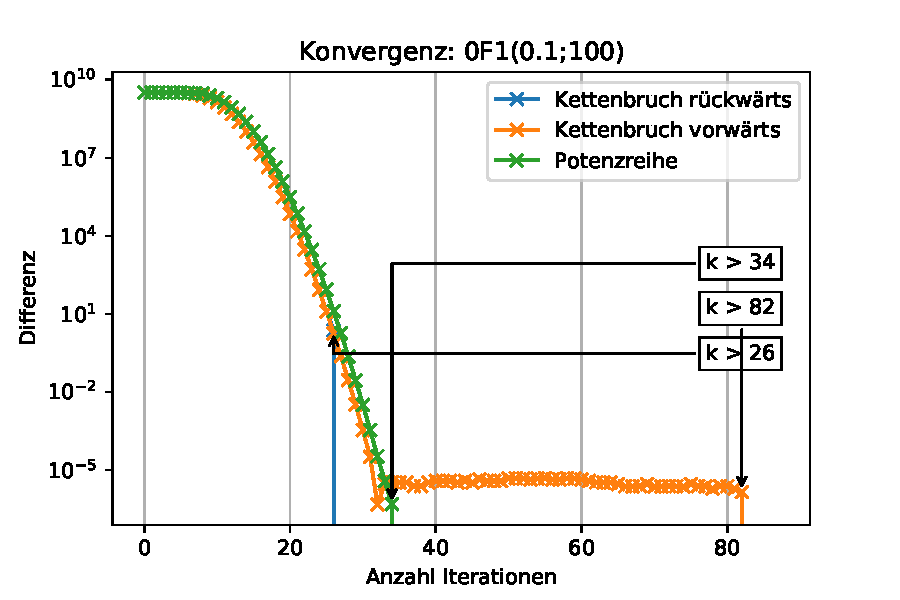
\includegraphics[width=0.8\textwidth]{papers/0f1/images/konvergenzPositiv.pdf}
    \caption{Konvergenz mit positivem z; Logarithmisch, vorzeichenlose dargestellte Differenz vom erwarteten Endresultat.
    \label{0f1:ausblick:plot:konvergenz:positiv}}
\end{figure}

\begin{figure}
    \centering
    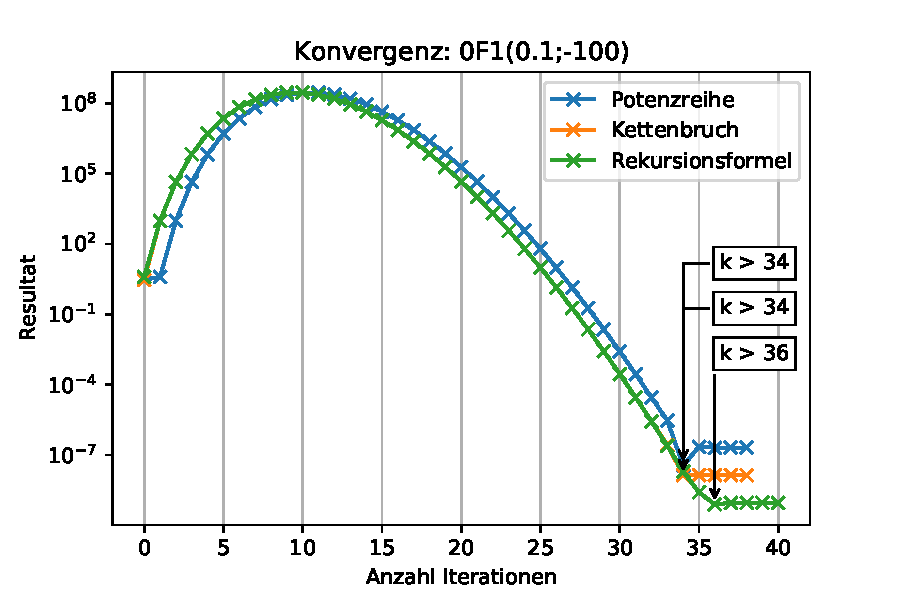
\includegraphics[width=0.8\textwidth]{papers/0f1/images/konvergenzNegativ.pdf}
    \caption{Konvergenz mit negativem z; Logarithmisch, vorzeichenlose dargestellte Differenz vom erwarteten Endresultat.
    \label{0f1:ausblick:plot:konvergenz:negativ}}
\end{figure}

\begin{figure}
    \centering
    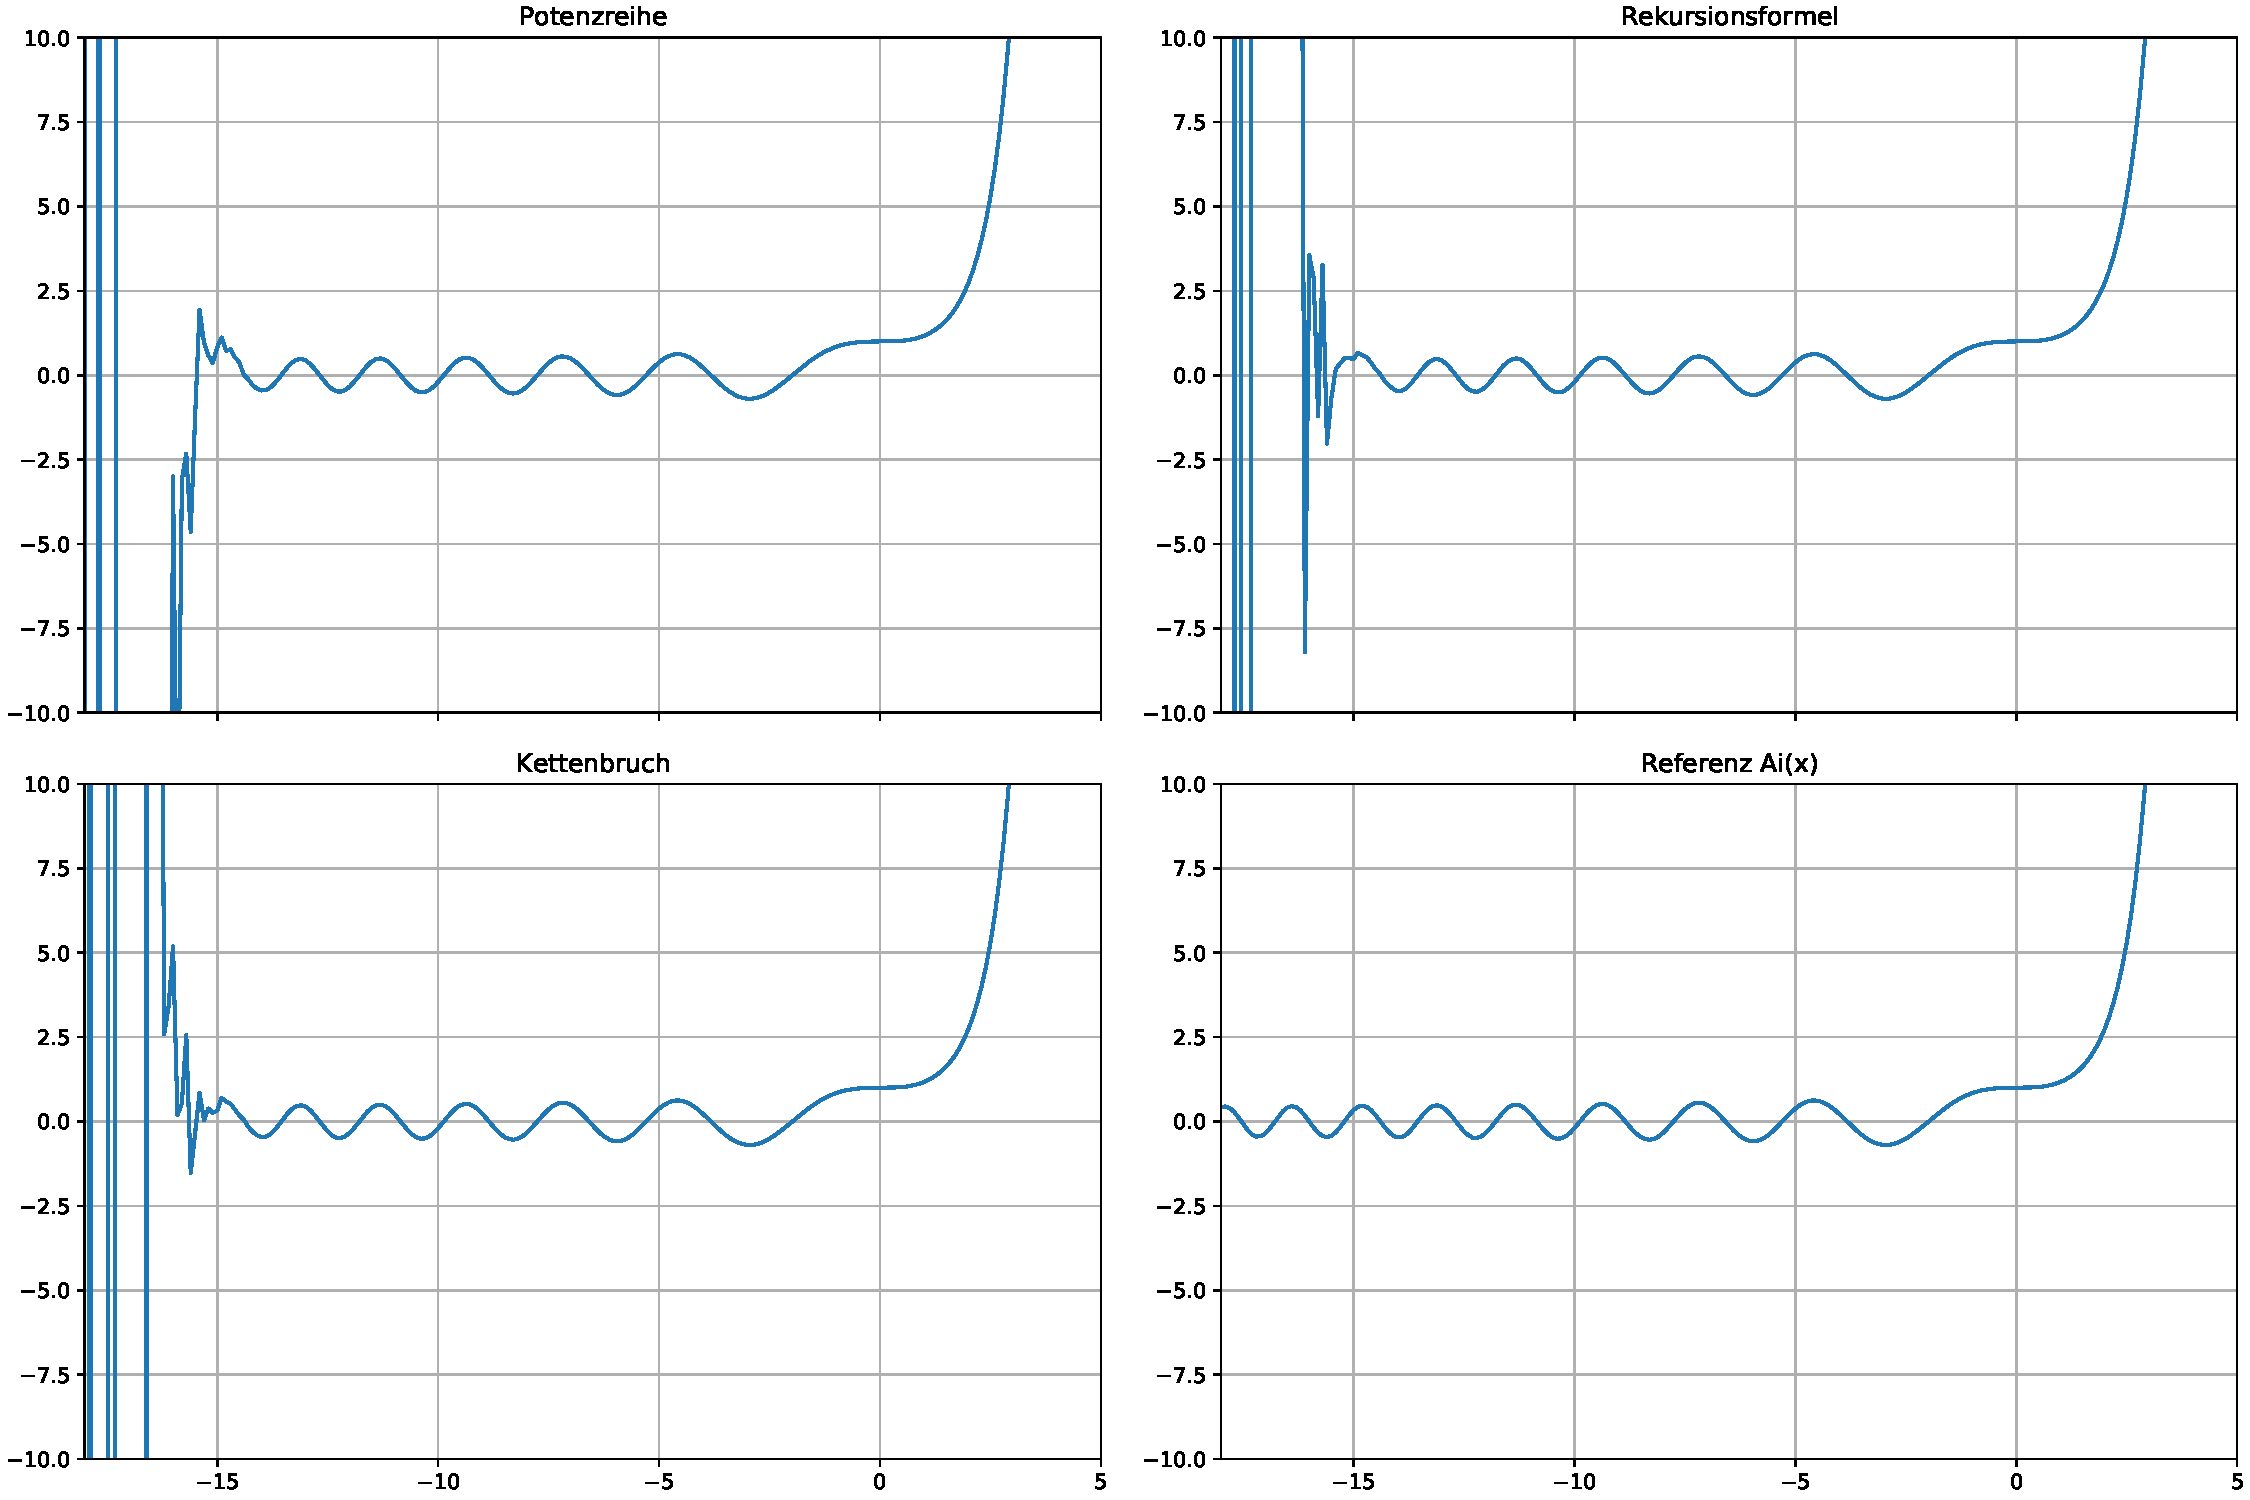
\includegraphics[width=1\textwidth]{papers/0f1/images/stabilitaet.pdf}
    \caption{Stabilität der 3 Algorithmen verglichen mit der Referenz Funktion $\operatorname{Ai}(x)$.
    \label{0f1:ausblick:plot:airy:stabilitaet}}
\end{figure}

